\section{Introduction}
\label{sec:introduction}

\begin{frame}{Why are we here?}
  \pause
  \begin{itemize}
    \item Probably because I asked you to come.
    \item Or because a professor told you to come.
  \end{itemize}
\end{frame}

\begin{frame}{Why are we here?}
  \begin{itemize}
    \item {\huge Model a nuclear reactor.}
      \pause
      \begin{itemize}
        \item Neutron distribution.
        \item Thermal Hydraulics.
        \item Thermal Expansion.
      \end{itemize}
  \end{itemize}
\end{frame}

\begin{frame}{But it's already been done!}
  \begin{itemize}
    \pause 
    \item You're right.
    \pause
    \item Computers are different now.
    \item Mathematical methods are more efficient now.
    \item \textbf{FORTRAN} has \textit{a few} new standards.
  \end{itemize}
\end{frame}

\begin{frame}{Present Simulation Procedure}
  \begin{itemize}
    \item Heuristically estimate material temperatures.
    \item Manually calculate thermally expanded dimensions.
    \item Manually calculate area fractions and number densities.
    \item Run \dif and get \keff and power distribution.
    \pause
    %\item \dif was last updated 1993. \textbf{FORTRAN} last updated 2008.
  \end{itemize}
  \vspace{0.3in}
  \begin{block}{}
    No thermal feedback capability. Modern numerical methods can be
    implemented.
  \end{block}
\end{frame}

\begin{frame}{Goals}
  \begin{itemize}
    \item User input.
      \begin{itemize}
        \item Easy to use.
        \item Reactor geometry via \texttt{VTK} mesh.
        \item Temperature dependent cross-sections either plain-text or 
          \texttt{ISOTXS}.
        \item Pin dimensions and material compositions.
      \end{itemize}
    \item Simulate thermal expansion and thermal hydraulics internally.
    \item Collect \keff, reactor power, and average material temperatures.
  \end{itemize}
  \vspace{0.25in}
  \begin{itemize}
    \item Thermal expansion and thermal hydraulic simulations have been moved
      internally and are now inherent to the simulation.
    \item Thermal hydraulic simulation also improves the accuracy of neutronics
      simulation by leading to more accurate cross sections.
  \end{itemize}
\end{frame}

\begin{frame}{Geometry Description}
  \begin{itemize}
    \item Hexagonal.
    \item Boxed assemblies.
    \item Resolve individual assemblies and specified elevations.
  \end{itemize}
\end{frame}

\begin{frame}{Fuel Rod}
  \begin{figure}
    \centering
    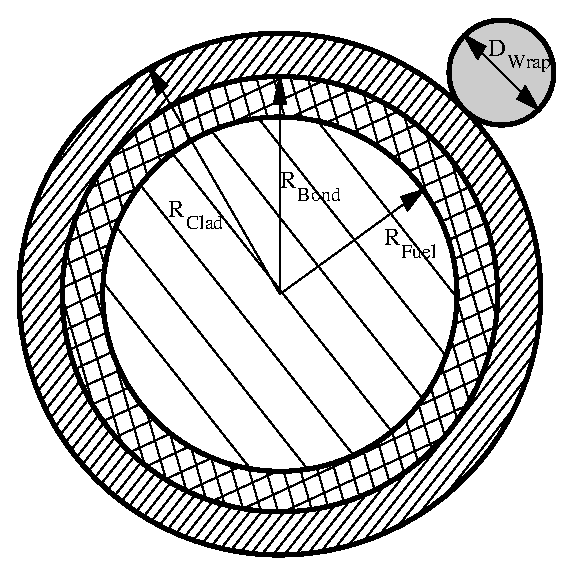
\includegraphics[width=0.5\textwidth]{pin_model}
    %\caption{Dimensions of Thermal Hydraulic Rod Model.}
    \label{fig:pin_model}
  \end{figure}
\end{frame}

\begin{frame}{Hexagonal Assembly}
  \begin{figure}
    \centering
    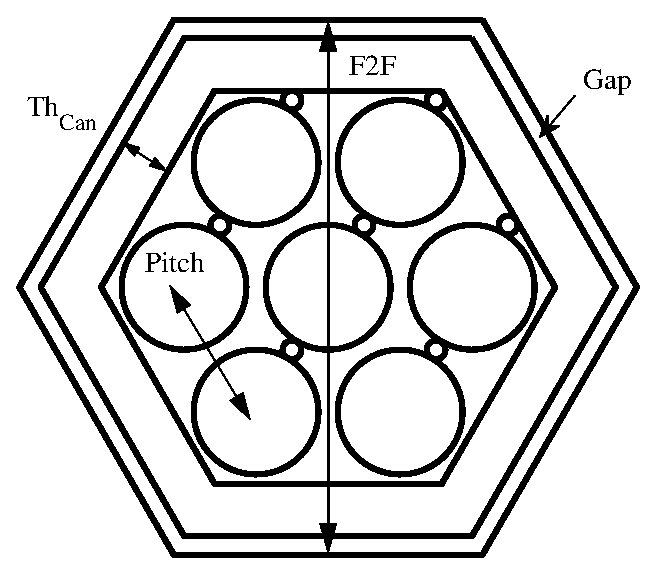
\includegraphics[width=0.5\textwidth]{hex_can}
    %\caption{Dimensions of Hexagonal Can.}
    \label{fig:hex_can}
  \end{figure}
\end{frame}

\begin{frame}{Fuel Assembly}
  \begin{figure}
    \centering
    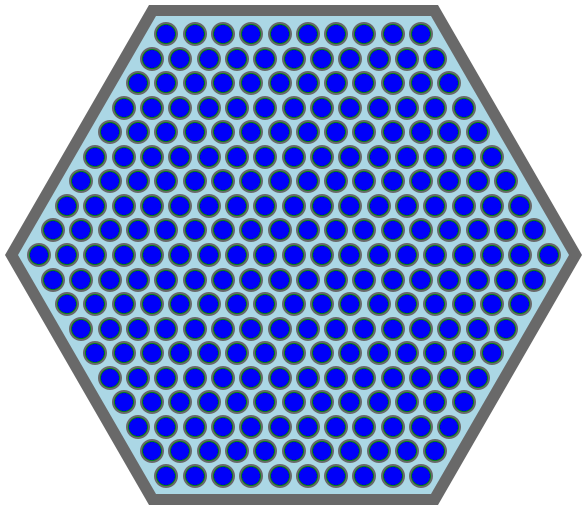
\includegraphics[width=0.5\textwidth]{prism_hex}
    \caption{Example of Fast Reactor Fuel Assembly Cross-section with 217 rods.}
    \label{fig:prism_hex}
  \end{figure}
\end{frame}

\begin{frame}
  \begin{figure}
    \centering
    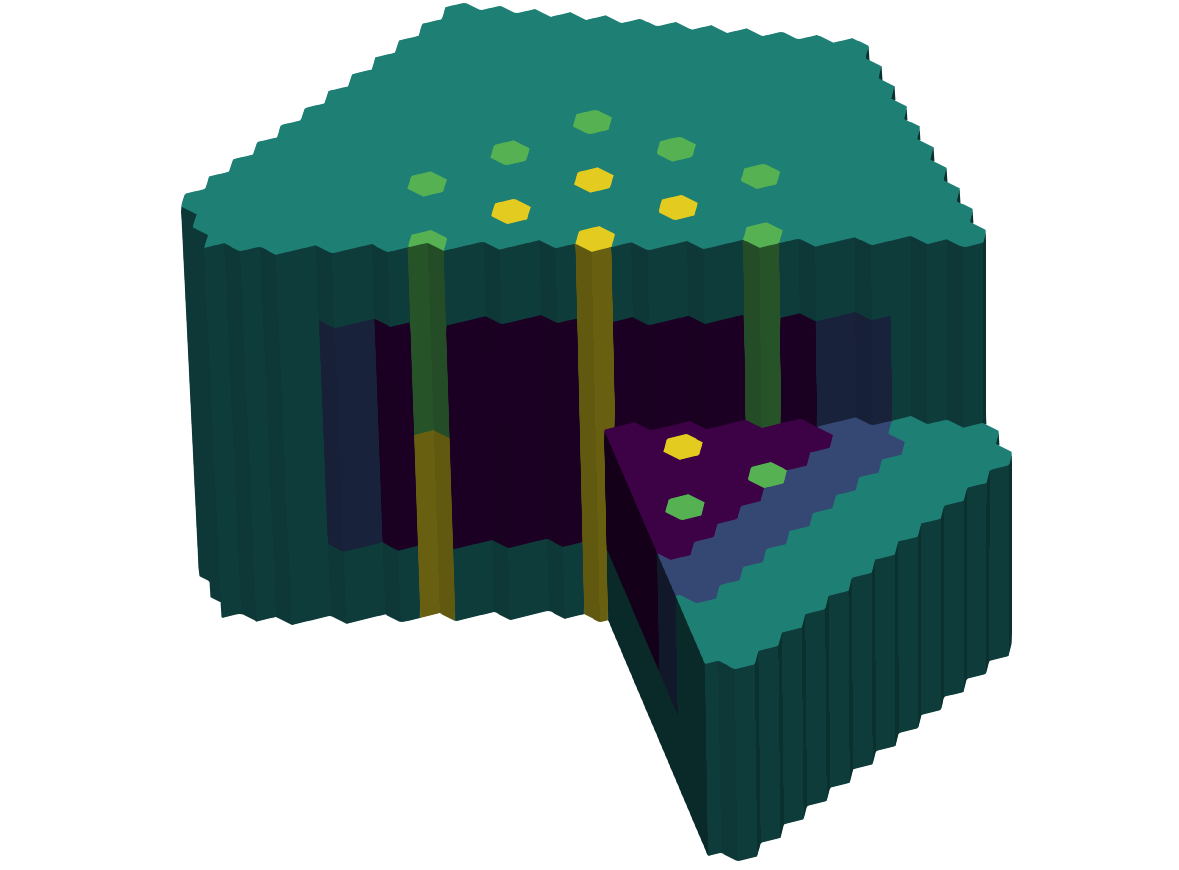
\includegraphics[width=0.9\textwidth]{reactor_materials}
    \caption{Example of Fast Reactor Materials based on MONJU.}
    \label{fig:reactor_materials}
  \end{figure}
\end{frame}
